\documentclass{article}

\usepackage[usenames,dvipsnames]{color}
\usepackage{hw}
\usepackage{bm}
\usepackage{amsmath}
\usepackage{graphicx}
\usepackage[colorlinks=true,urlcolor=blue]{hyperref}
\usepackage{geometry}
\geometry{margin=1in}
\usepackage{float}
\setlength{\marginparwidth}{2.15cm}
\usepackage{booktabs}
\usepackage{enumitem}
\usepackage{epsfig}
\usepackage{setspace}
\usepackage{parskip}
\usepackage[]{algorithm2e}
\usepackage{comment}
\usepackage{pdfpages}
\usepackage{physics}
\usepackage{hyperref}
\usepackage{macro}
\newcommand{\st}{\mathop{\mathrm{subject\,\,to}}}

\usepackage{listings}
\usepackage{color}

\definecolor{codegreen}{rgb}{0,0.6,0}
\definecolor{codegray}{rgb}{0.5,0.5,0.5}
\definecolor{codepurple}{rgb}{0.58,0,0.82}
\definecolor{backcolour}{rgb}{0.95,0.95,0.92}

\lstdefinestyle{mystyle}{
	backgroundcolor=\color{backcolour},   
	commentstyle=\color{codegreen},
	keywordstyle=\color{magenta},
	numberstyle=\tiny\color{codegray},
	stringstyle=\color{codepurple},
	basicstyle=\footnotesize,
	breakatwhitespace=false,         
	breaklines=true,                 
	captionpos=b,                    
	keepspaces=true,                 
	numbers=left,                    
	numbersep=5pt,                  
	showspaces=false,                
	showstringspaces=false,
	showtabs=false,                  
	tabsize=2
}

\lstset{style=mystyle}


%\newcommand{\comment}[1]{\textcolor{blue}{\textsc{\textbf{[#1]}}}}


\makeatletter
\newcommand{\removelatexerror}{\let\@latex@error\@gobble}
\makeatother

\begin{document}

\section*{}
\begin{center}
  \centerline{\textsc{\LARGE Homework 3}}
  \vspace{0.5em}
  \centerline{\textsc{\Large Decision Tree, KNN, Kernel SVM}}
  \vspace{1em}
  \textsc{\large CMU 10-701: Machine Learning (Spring 2017)} \\
  \vspace{1em}
  \centerline{OUT: Feb 27}
  \centerline{DUE: March 10, 11:59 PM}
\end{center}
\graphicspath{images}

\section*{START HERE: Instructions}


\begin{itemize*}

\item \textbf{Collaboration policy:} Collaboration on solving the homework is allowed, after you have thought about the problems on your own.  It is also OK to get clarification (but not solutions) from books or online resources, again after you have thought about the problems on your own.  There are two requirements: first, cite your collaborators fully and completely (e.g., ``Jane explained to me what is asked in Question 3.4'').  Second, write your solution {\em independently}: close the book and all of your notes, and send collaborators out of the room, so that the solution comes from you only.



\item\textbf{Submitting your work:} Assignments should be submitted as PDFs using Gradescope unless explicitly stated otherwise.  Each derivation/proof should be completed on a separate page. Submissions can be handwritten, but should be labeled and clearly legible.  Else, submissions can be written in LaTeX.  Upon submission, label each question using the template provided by Gradescope.

 \item \textbf{Programming}: All programming portions of the assignments should be submitted to Gradescope as well.  We will not be using this for autograding, but rather for plagiarism detection, meaning you may use any language which you like to submit.
\end{itemize*}

\newpage

\section*{Section A : Multiple Choice Questions [10 points] (Dan)}

\begin{enumerate}
	\item {\textbf{[2 points]} Suppose that you are using ridge regression to estimate the relationship between your data and a value of interest. Your estimate for $\hat{\beta}$ is given by:
	$$\hat{\beta} = \argmin_\beta \norm{y - X \beta}_2^2 + \lambda \norm{\beta}_2^2$$
	Where $\lambda$ is a hyper-parameter that governs how much to penalize model complexity. Which of the following would be valid ways to use a 10-fold cross validation scheme? Select all that apply.
	}
	\begin{enumerate}[label=\Alph*)]
			\item {
				 For different values of $\lambda$, train on 9 of the folds and estimate the risk on the 10th fold. Select $\lambda$ by using the value that has the lowest risk on this 10th fold. Repeat this procedure 10 times for each possible hold out and use the mean of the risks for the estimators selected at each round as an estimate of the true risk of the model.
			}
			\item {
				 For different values of $\lambda$, train on 8 of the folds and estimate the risk on the 9th fold. Select $\lambda$ by using the value that has the lowest risk on this 9th fold. Then estimate the risk using this $\lambda$ on the 10th fold. Repeat this procedure 45 (10 choose 2) times and use the mean of the risks for the estimators selected each round as an estimate of the true risk of the model.
			}
			\item {
				 For different values of $\lambda$, train on 1 of the folds, and estimate the risk on this same fold. Select $\lambda$ by using the value that has the lowest risk on this fold. Repeat this procedure 10 times (once for each fold), and use the mean of the risks for the estimators as an estimate of the true risk of the model.
			}
			\item {
				 Select a value of $\lambda$ before doing your experiment. Train on 9 of the folds and estimate the risk on the 10th fold. Repeat this procedure 10 times (once for each fold), and use the mean of the risks for the estimators as an estimate of the true risk of the model.
			}
	\end{enumerate}
	\textbf{Answer:}\underline{D}\\
	To estimate the true risk from a CV, a fix $\lambda$ should be selected first.
	
	\item {\textbf{[2 points]} For a k-Nearest Neighbor classifier and the data set below, which class will the test point (marked by the black circle) be  classified as for each of the following values of $k$? \\
	\begin{minipage}[!ht]{0.5\textwidth}
			\centering
			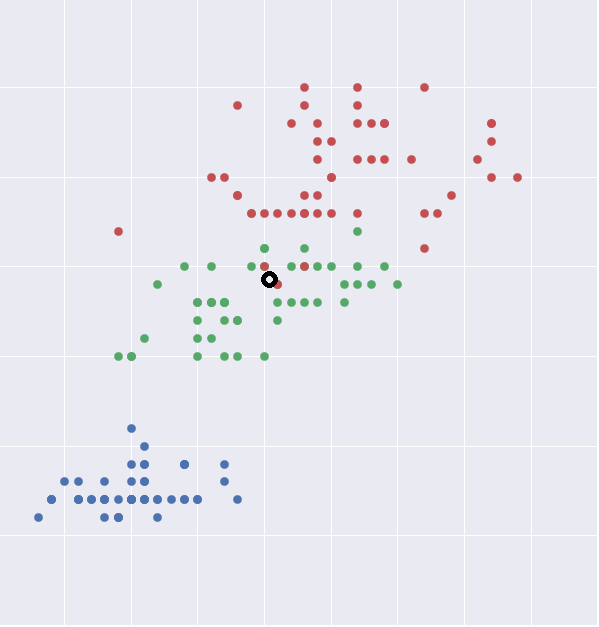
\includegraphics[width=1.0\textwidth]{knn_test_point.png}
			\label{fig:knn_test_point}
		\end{minipage}
	\begin{minipage}[!ht]{0.25\textwidth}
		\begin{enumerate}[label=(\roman*)]
			\item $k = 1$ \textbf{Answer:}\underline{A}
			\item $k = 2$ \textbf{Answer:}\underline{A}
			\item $k = 7$ \textbf{Answer:}\underline{B}
		\end{enumerate}
	\end{minipage}
	\begin{minipage}[!ht]{0.25\textwidth}
		\begin{enumerate}[label=\Alph*)]
			\item Red
			\item Green
			\item Blue
		\end{enumerate}
	\end{minipage}
	}
	
	\item {\textbf{[2 points]} Which of the following statements is true about the k-Nearest Neighbor classifier? Select all that apply.
		\begin{enumerate}[label=\Alph*)]
			\item{ As the value of $k$ increases, the variance of the model increases }
			\item{ As the value of $k$ increases, the bias of the model increases }
			\item{ As the value of $k$ increases, the model complexity increases }
			\item{ As the value of $k$ increases, the number of parameters in the model increases }
			\item{ As the number of training data points increases, the memory requirements of the model increase }
		\end{enumerate}
	}
	\textbf{Answer:}\underline{B, E}\\
	\begin{itemize}
		\item For A: the variance of the model will decrease
		\item For C: the model complexity will decrease
		\item For D: the number of parameters in the model will not change
	\end{itemize}
	
	
	\item {\textbf{[2 points]} What is the maximum training error for a decision tree on an arbitrary data set with $k$ discrete output classes?
	
		\begin{enumerate}[label=\Alph*)]
			\item $\frac{1}{k}$
			\item $1$
			\item $\frac{1}{\log_2{k}}$
			\item $\frac{k - 1}{k}$
		\end{enumerate}
	
	}
	\textbf{Answer}:\underline{D}\\
	This may happen when $P(Y)=P(Y|X_i),~\forall i$, and all data will be in a leaf node with a class label whose prior $P(Y)$ is the highest. To maximize the training error, the minimum training accuracy will be $1/k$; therefore, the maximum training error is $(k-1)/k$
	
	\item {\textbf{[2 points]} Consider the following data set. Which methods will classify all data points in this set correctly? Select all that apply. \\
		\begin{minipage}[!ht]{0.5\textwidth}
			\centering
			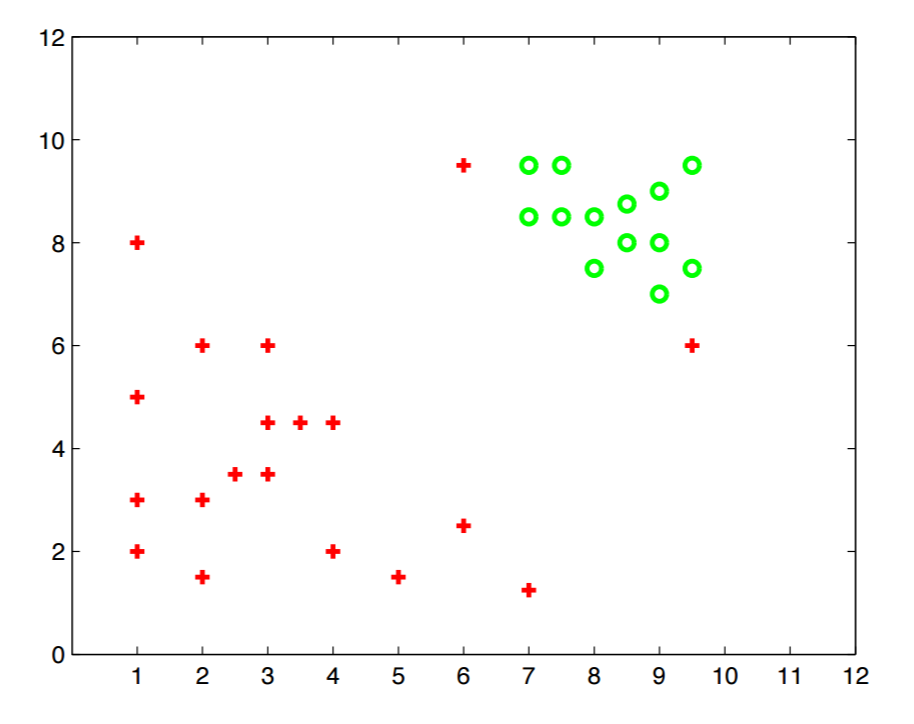
\includegraphics[width=1.0\textwidth]{mcq_data.png}
			\label{fig:svm_quad_a}
		\end{minipage}
		\begin{minipage}[!ht]{0.5\textwidth}
			\begin{enumerate}[label=\Alph*)]
				\item Soft-Margin SVM (with no kernel)
				\item SVM with a quadratic kernel, when the coefficient on the penalty for slack variables $C = 0$
				\item SVM with a quadratic kernel, when the coefficient on the penalty for slack variables $C \rightarrow \infty$
				\item Logistic regression (no kernel)
				\item 3-NN
			\end{enumerate}
		\end{minipage} 
	}
	\textbf{Answer}:\underline{C}\\
	\begin{itemize}
		\item For A: The data is not linear separable. Two outlier red points will be misclassified.
		\item For B: Because $C=0$, there will be no classification at all.
		\item For C: $C\rightarrow \infty$ means hard-margin SVM is used. The quadratic kernel is used, and the data is non-linear separable.
		\item For D: Logistic is linear classifier.
		\item For E: The two outlier red points will be misclassified.
	\end{itemize}
	
\end{enumerate}

\newpage


\section*{Part B, Problem 1: Decision Tree (30 pts) (Hao and Yiting)}

\subsection*{1.1 Build Your Own Decision Tree (14 pts)}

The following is a small synthetic data set where we try to predict the usage of individual mobile phones based on their income, age, education, and marital status. In this section, you can assume that the decision tree is built using the ID3 algorithm, where each attribute is used only as an internal node.


\begin{center}
  \begin{tabular}{ l l l l | l }
    \hline
    Income & Age & Education & Martial Status & Usage \\ \hline \hline
    Low & Old & University & Married & Low \\ \hline
    Medium & Young & College & Single & Medium  \\ \hline
    Low & Old & University & Married & Low  \\ \hline
    High & Young & University & Single & High  \\ \hline
    Low & Old & University & Married & Low  \\ \hline
    High & Young & College & Single & Medium  \\ \hline
    Medium & Young & College & Married & Medium  \\ \hline
    Medium & Old & High School & Single & Low  \\ \hline
    High & Old & University & Single & High  \\ \hline
    Low & Old & High School & Married & Low  \\ \hline
    Medium & Young & College & Married & Medium  \\ \hline
    Medium & Old & High School & Single & Low  \\ \hline
    High & Old & University & Single & High  \\ \hline
    Low & Old & High School & Married & Low  \\ \hline
    Medium & Young & College & Married & Medium  \\ \hline
  \end{tabular}
\end{center}

\begin{enumerate}

\item\textbf{[2 points]} What is the initial entropy of Usage?
\\\textbf{Answer:}\\
Usage:
\begin{itemize}
	\item Low: 7
	\item Medium: 5
	\item High: 3
\end{itemize}
Therefore,
$$H(Y)=-\frac{7}{15}\log_2\frac{7}{15}-\frac{5}{15}\log_2\frac{5}{15}-\frac{3}{15}\log_2\frac{3}{15}=1.506$$

\item\textbf{[5 points]} Which attribute should be chosen at the root of the tree? Show your calculation for the information gains (IG) and explain your choice in a sentence.
\\\textbf{Answer:}\\
\begin{itemize}
	\item Income:
	\begin{itemize}
		\item Low: 5 (L: 5, M: 0, H: 0)
		$$P(Low)H(Y|Low)=-\frac{5}{15}(\frac{5}{5}\log_2\frac{5}{5}+\frac{0}{5}\log_2\frac{0}{5}+\frac{0}{5}\log_2\frac{0}{5})=0.000$$
		\item Medium: 6 (L: 2, M: 4, H: 0)
		$$P(Medium)H(Y|Low)=-\frac{6}{15}(\frac{2}{6}\log_2\frac{2}{6}+\frac{4}{6}\log_2\frac{4}{6}+\frac{0}{6}\log_2\frac{0}{5})=0.367$$
		\item High: 4 (L: 0, M: 1, H: 3)
		$$P(Medium)H(Y|High)=-\frac{4}{15}(\frac{0}{4}\log_2\frac{0}{4}+\frac{1}{4}\log_2\frac{1}{4}+\frac{3}{4}\log_2\frac{3}{4})=0.216$$
	\end{itemize}
	$$IG(Y;Income)=H(Y)-H(Y|Income)=1.506-0.000-0.367-0.216=0.923$$
	\item Age:
	\begin{itemize}
		\item Young: 6 (L: 0, M: 5, H: 1)
		$$P(Young)H(Y|Young)=-\frac{6}{15}(\frac{0}{6}\log_2\frac{0}{6}+\frac{5}{6}\log_2\frac{5}{6}+\frac{1}{6}\log_2\frac{1}{6})=0.260$$
		\item Old: 9 (L: 7, M: 0, H: 2)
		$$P(Old)H(Y|Old)=-\frac{9}{15}(\frac{7}{9}\log_2\frac{7}{9}+\frac{0}{9}\log_2\frac{0}{9}+\frac{2}{9}\log_2\frac{2}{9})=0.459$$
	\end{itemize}
	$$IG(Y;Age)=H(Y)-H(Y|Age)=1.506-0.260-0.459=0.787$$
	\item Education:
	\begin{itemize}
		\item High School: 4 (L: 4, M: 0, H: 0)
		$$P(High School)H(Y|High School)=-\frac{4}{15}(\frac{4}{4}\log_2\frac{4}{4}+\frac{0}{4}\log_2\frac{0}{4}+\frac{0}{4}\log_2\frac{0}{4})=0.000$$
		\item College: 5 (L: 0, M: 5, H: 0)
		$$P(College)H(Y|College)=-\frac{5}{15}(\frac{0}{5}\log_2\frac{0}{5}+\frac{5}{5}\log_2\frac{5}{5}+\frac{0}{5}\log_2\frac{0}{5})=0.000$$
		\item University: 6 (L: 3, M: 0, H: 3)
		$$P(University)H(Y|University)=-\frac{6}{15}(\frac{3}{6}\log_2\frac{3}{6}+\frac{0}{6}\log_2\frac{0}{6}+\frac{3}{6}\log_2\frac{3}{6})=0.400$$
	\end{itemize}
	$$IG(Y;Education)=H(Y)-H(Y|Education)=1.506-0.000-0.000-0.400=1.106$$
	\item Martial Status:
	\begin{itemize}
		\item Single: 7 (L: 2, M: 2, H: 3)
		$$P(Single)H(Y|Single)=-\frac{7}{15}(\frac{2}{7}\log_2\frac{2}{7}+\frac{2}{7}\log_2\frac{2}{7}+\frac{3}{7}\log_2\frac{3}{7})=0.726$$
		\item Married: 8 (L: 5, M: 3, H: 0)
		$$P(Married)H(Y|Married)=-\frac{8}{15}(\frac{5}{8}\log_2\frac{5}{8}+\frac{3}{8}\log_2\frac{3}{8}+\frac{0}{8}\log_2\frac{0}{8})=0.509$$
	\end{itemize}
	$$IG(Y;Martialtion)=H(Y)-H(Y|Martial)=1.506-0.726-0.509=0.271$$
\end{itemize}
Because $IG(Y;Education)$ is the largest information gain, the ``Education" attribute should be chosen at the root of the tree.

\item\textbf{[7 points]} Draw the full decision tree for the data.
\\\textbf{Answer:}\\
\begin{itemize}
	\item Education = High School $\Rightarrow$ Usage = Low
	\item Education = College $\Rightarrow$ Usage = Medium
	\item Education = University
	\begin{itemize}
		\item Martial Status = Married $\Rightarrow$ Usage = Low
		\item Martial Status = Single $\Rightarrow$ Usage = High
	\end{itemize}
\end{itemize}

\end{enumerate}


\subsection*{1.2 Decision Tress Analysis (16 pts)}

\begin{enumerate}

\item\textbf{[8 points]} Suppose $X$ and $Y$ are discrete variables. Let $IG$ be the information gain and $H$ be the entropy. Show that $IG(X;Y) = H(X,Y) - H(X|Y) - H(Y|X).$
\\\textbf{Answer:}\\
\begin{equation}
\nonumber
\begin{array}{rcl}
IG(X;Y) & = & H(Y) - H(Y|X) \\
		& = & -\sum_y P(y)\log_2P(y) + \sum_x P(x) \sum_y P(y|x)\log_2P(y|x) \\
		& = & -\sum_{x,y} P(x,y)\log_2P(y) -\sum_{x,y} P(x,y)\log_2P(x|y) \\
		&   & +\sum_{x,y} P(x,y)\log_2P(x|y) +\sum_{x,y} P(x,y)\log_2P(y|x) \\
		& = & -\sum_{x,y} P(x,y)\log_2P(x,y) \\
		&   & + \sum_y P(y) \sum_x P(x|y)\log_2P(x|y) + \sum_x P(x) \sum_y P(y|x)\log_2P(y|x) \\
		& = & H(X,Y) - H(X|Y) - H(Y|X)
\end{array}
\end{equation}

\item\textbf{[4 points]} Occam's Razor can be interpreted as simpler hypotheses are generally better than the complex ones. Does ID3 follow Occam's Razor? How about C4.5? Explain briefly (no more than 3 sentences).
\\\textbf{Answer:}\\
The ID3 does not follow Occam's Razor, and C4.5 follows Occam's Razor, because the C4.5 has an additional step to prune back tree to reduce over-fitting and get simpler hypotheses.

\item\textbf{[4 points]} Consider a decision tree $T$ learned on a training set of $n$ instances. Assume that there are two identical instances $X$ and $X\prime$ (i.e. they have exactly the same attributes and labels) in the training set. Can removing $X\prime$ out of the training set produce a different $T$? Explain Briefly (no more than 4 sentences).
\\\textbf{Answer:}\\
Yes, the tree may change, because decision tree classifier requires the availability of all training data to build the tree. E.g. the mid-points of features in C4.5 may change even we just remove a duplicated point.

\end{enumerate}


\newpage


\section*{Part B, Problem 2 K-NN (15 pts) (Weixiang)}
\begin{enumerate}
	\item \textbf{(9 points)}
	For each of the following figures, we are given a few data points in
	2-d space,each of which is labeled as either positive (blue) or
	negative (red). Assuming that we are using L2 distance as a distance
	metric, draw the decision boundary for 1-NN for each case. In other words, with your decision boundary, the new test data can be classified into corresponding categories. As an example, we draw the decision boundary for you with figure (a).
	
	\begin{figure*}[h!]
		\centering
		\begin{tabular}{cccc}
			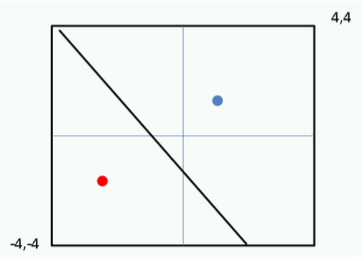
\includegraphics[width=.25\columnwidth]{pa.png}& 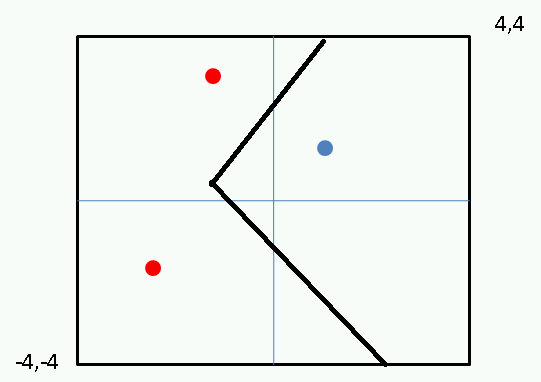
\includegraphics[width=.25\columnwidth]{pb.png}& 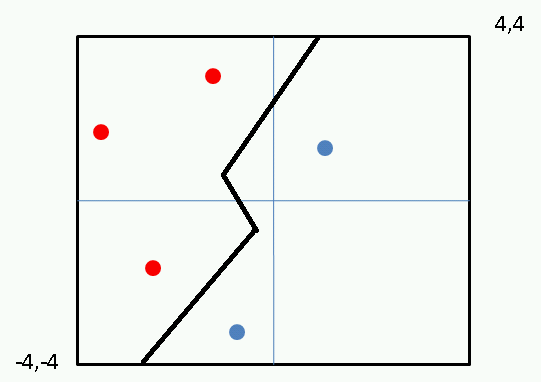
\includegraphics[width=.25\columnwidth]{pc.png}&
			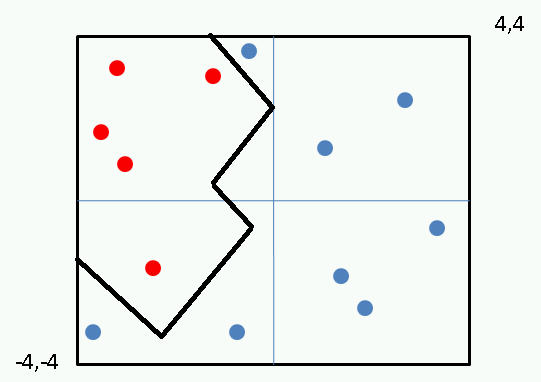
\includegraphics[width=.25\columnwidth]{pd.png}\\
			(a) & (b) & (c) & (d)
		\end{tabular}
	\end{figure*}
	
	
	\item \textbf{(3 points)} In class we have mentioned that K-NN is a \emph{lazy}
	classifier. Do we \emph{always} need to store all training data to build our 1-NN classifier when we have $n (n\geq3)$ points? Why? Is there a case that you must store all training data points (i.e., use all training data points when doing the classification)? Why?
	\\\textbf{Answer:}\\
	No, we don't need to store all data points for 1-NN classifier, because if we draw a Veronoi diagram for all points, then the point that only has same labeled neighbors can be omitted. If all points have differently labeled neighbors, all points should be stored. 
	
	\item \textbf{(3 point)}
	Decision tree classfier requires the availability of all training data to build the tree. Thus when a new training data point comes in, it might influence the structure of the decision tree. Does K-NN also suffer from this problem and why (explian in 1-2 sentences)? 
	\\\textbf{Answer:}\\
	With the increment of K, the decision boundary relies on more and more training data and even the whole dataset. If this happens, K-NN may also suffers from this problem.
	
\end{enumerate}
\newpage


\section*{Part B, Problem 3: Kernel SVM (15 pts) (Adams)}
After Homework 2, you must be very familiar with SVM.
In this question, we are considering its Kernel version:
\begin{align*}
\min_{w\in \mathbb{R}^d, b, \xi_i\in\mathbb{R},i=1,2,...,n} &\quad \frac{1}{2}||w||_2^2 + C\sum_{i=1}^n\xi_i\\
\text{s.t.} &\quad y^{(i)}(w^\mathsf{T}\phi(x^{(i)}) + b) \geq 1-\xi_i,~~  \forall i = 1,\ldots, n\\
 &\quad \xi_i \geq 0, ~~ \forall i = 1,\ldots, n
\end{align*}
where $x^{(i)}\in\mathbb{R}^p, i=1,2,...,n$ is the original training data coming along with the label $y^{(i)}\in\{-1,1\}$, $C>0$ is a constant and $\phi: \mathbb{R}^p \rightarrow \mathbb{R}^d$ is a mapping function that maps the original data to a new space. Generally speaking, $d>p$ (In fact, $d$ can be $+\infty$). Please answer the following questions. Note that the questions with complexity could be answered with big-O notation.

\begin{enumerate}
\item \textbf{[6 points]} First write down the Lagrangian of the above problem and then derive the dual problem step by step.
\\\textbf{Answer:}\\

$$J(\vec{w},b,\vec{\xi},\vec{\alpha},\vec{\gamma}) = \frac{1}{2}\vec{w}^T\vec{w}+C\sum_{i=1}^{n}\xi_i + \sum_{i=1}^{n} \alpha_i(1-\xi_i-y^{(i)}(\vec{w}^T\phi(\vec{x}^{(i)})+b)) - \sum_{i=1}^{n}\gamma_i\xi_i~~~~(\alpha_i\geq0,~\gamma_i\geq0)$$

Because,
\begin{equation}
\nonumber
\begin{array}{rcl}
\left.\frac{\partial J}{\partial \vec{w}}\right|_{\vec{w}^*} & = & \vec{w}^*-\sum_{i=1}^{n}\alpha_iy^{(i)}\phi(\vec{x}^{(i)}) = 0 \\
									& \Rightarrow & \vec{w}^* = \sum_{i=1}^{n}\alpha_iy^{(i)}\phi(\vec{x}^{(i)}) \\

\left.\frac{\partial J}{\partial b}\right|_{b^*} & = & -\sum_{i=1}^{n}\alpha_iy^{(i)} = 0 \\
& \Rightarrow & \sum_{i=1}^{n}\alpha_iy^{(i)} = 0 \\	

\left.\frac{\partial J}{\partial \xi_i}\right|_{\xi_i^*} & = & C-\alpha_i-\gamma_i = 0 \\
& \Rightarrow & C = \alpha_i+\gamma_i \\								
\end{array}
\end{equation}
Therefore,
$$J(\vec{w}^*,b^*,\vec{\xi}^*,\vec{\alpha},\vec{\gamma}) = -\frac{1}{2}\sum_{i=1}^{n}\sum_{j=1}^{n}\alpha_i\alpha_j y^{(i)} y^{(j)} \phi^T(\vec{x}^{(i)})\phi(\vec{x}^{(j)})+\sum_{i=1}^{n}\alpha_i$$
Therefore, the dual form is:
$$\max_{\vec{\alpha},\vec{\gamma}} -\frac{1}{2}\sum_{i=1}^{n}\sum_{j=1}^{n}\alpha_i\alpha_j y^{(i)} y^{(j)} \phi^T(\vec{x}^{(i)})\phi(\vec{x}^{(j)})+\sum_{i=1}^{n}\alpha_i$$
s.t.
$$\sum_{i=1}^{n}\alpha_i y^{(i)} = 0$$
$$0\leq\alpha_i\leq C$$


\item \textbf{[9 points, (3 for each subproblem)]} Suppose we have obtained the solution of the dual problem, which is denoted as $\alpha_i^*$ for $i=1,2,...,n$. Please find out the corresponding primal solution $w^*$ and $b^*$ in the course slides. Given a test data point $z\in \mathbb{R}^p$,
\\\textbf{Answer:}\\
$$\vec{w}^* = \sum_{i=1}^{n}\alpha_i^*y^{(i)}\phi(\vec{x}^{(i)})$$
$$b^* = y^{(k)}-\sum_{i=1}^{n}\alpha_i^*y^{(i)}\phi^T(\vec{x}^{(i)})\phi(\vec{x}^{(k)})~~~~(for~any~k~where~C>\alpha_k>0)$$

\begin{itemize}
\item What is the time complexity of making the classification decision if the mapping is given by $$\phi(x) = (\underbrace{x_p^2, x_{p-1}^2, ..., x_1^2}_{p}, \underbrace{ \sqrt{2}x_{p}x_{p-1},..., \sqrt{2}x_{p}x_{1}}_{p-1}, \underbrace{\sqrt{2}x_{p-1}x_{p-2},...,\sqrt{2}x_{p-1}x_{1}}_{p-2},...,\sqrt{2}x_{2}x_{1}, \sqrt{2c}x_{p},...,\sqrt{2c}x_{1}, c)^\mathsf{T}$$
with a constant $c>0$ and we need to compute it from scratch?
\\\textbf{Answer:}\\
\begin{itemize}
	\item For $\phi(\vec{x}^{(i)})$: the number of multiply operations is $n\frac{(p+2)(p+1)}{2}$
	\item For $\vec{w}^*$: the number of multiply operations is $n\frac{(p+2)(p+1)}{2}$
	\item For $b^*$: the number of multiply operations is $2n\frac{(p+2)(p+1)}{2}$
	\item For $\phi(\vec{z})$: the number of multiply operations is $\frac{(p+2)(p+1)}{2}$
	\item For $sgn(\vec{w}^*\cdot\phi(\vec{z})+b)$:	the number of multiply operations is $\frac{(p+2)(p+1)}{2}$
	\item Therefore, the time complexity is $O(np^2)$
\end{itemize}

\item  Let $K(u,v) = \phi(u)^\mathsf{T}\phi(v)$ where $\phi(\cdot)$ has the same definition as above. Please give a compact form of $K(u,v)$. What is the time complexity of making the classification decision if we directly compute $K(\cdot, \cdot)$?
\\\textbf{Answer:}\\
$$K(\vec{u},\vec{v}) = \phi(\vec{u})^T\phi(\vec{v}) = (\vec{u}^T\vec{v}+C)^2$$
\begin{itemize}
	\item For $\vec{w}^*\cdot\phi(\vec{z})=\sum_{i=1}^{n}\alpha_iy_iK(\vec{z},\vec{x}_i)$: the number of multiply operations is $n(p+2)$
	\item For $b^*=y_k-\sum_{i=1}^{n}\alpha_iy_iK(\vec{x}_k,\vec{z})$: the number of multiply operations is $n(p+2)$
	\item For $sgn(\vec{w}^*\cdot\phi(\vec{z})+b)$:	the number of multiply operations is $0$
	\item Therefore, the time complexity is $O(np)$
\end{itemize}

\item Now please go back to the dual formulation you derived previously. To avoid repetitive computation, one can precompute all the inner products $K(x^{(i)},x^{(j)})=\phi(x^{(i)})^\mathsf{T}\phi(x^{(j)})$ before solving the dual problem. What is the space complexity of this approach and what might be a problem if $n$ is huge?
\\\textbf{Answer:}\\
The space complexity of $K(x^{(i)},x^{(j)})$ is $O(n^2)$, and this may lead memory overflow if $n$ is huge.

\end{itemize}
\end{enumerate}

\newpage

\newpage

\section*{Part C: Implementing SVM Variation [20 points] (Yichong and Prakhar) }
\textbf{Please attach your code as appendix to this problem.}\\
In the last homework, we derived a variant of SVM that explicitly maximizes the margin.
You can use any library on quadratic optimization (e.g., CVXOPT for python or \textsf{quadprog} for MATLAB) for this problem. Here is an instruction on CVXOPT.

Installation instructions of CVXOPT can be found \href{http://cvxopt.org/install/index.html}{here}. CVXOPT provides an easy interface for quadratic programming: The function \textsf{qp(P, q[, G, h[, A, b]])} solves the optimization problem
\begin{align*}
\text{minimize}_{x \in \mathbb{R}^n}\;  & (1/2) x^TPx+q^Tx \\
\text{subject to } & Gx \preceq h \\
& Ax=b
\end{align*}
for $P\in \mathbb{R}^{n\times n}, q\in \mathbb{R}^n, G\in \mathbb{R}^{m_1\times n}, h \in \mathbb{R}^{m_1}, A \in \mathbb{R}^{m_2\times n}, b \in \mathbb{R}^{m_2}$.
Here $\preceq$ means pointwise less than or equal; i.e., if $a \preceq b $ for $a,b \in \mathbb{R}^n$, then $a_i\leq b_i \forall i=1,2,...,n$, where the subscript indicates coordinates. Look into \href{http://cvxopt.org/examples/tutorial/qp.html}{here} for a concrete example including all details.

In last homework we want to solve the following primal problem:
\begin{align}
\min_{\boldsymbol{w}, \boldsymbol{\xi}, \rho}&\quad \frac{1}{2} {\boldsymbol{||w||}}_2^2 + \frac{1}{2}b^2- \rho + \frac{\lambda}{2} \sum_{i=1}^n \xi_i^2\label{eqn:primal}\\
\text{subject to} &\quad y_i(w^T \boldsymbol{x_i} + b) \ge \rho - \xi_i,\quad i = 1,\dotsc,n 	\nonumber
\end{align}


We derived a dual program of (\ref{eqn:primal}) in homework 2. (Have a look at the solutions if you did not solve it - we will release it soon.) Implement the dual program using CVXOPT. Compute results for both $\lambda=1$ and $\lambda=10$. The data is a toy dataset *train\_data.csv* in {\color{red}csv} format of size $\mathbb{R}^{100\times 2}$, and the training label is contained in the file *train\_label.csv* of size $\mathbb{R}^{100\times 1}$. Be careful that CVXOPT uses a slightly different matrix format than numpy; so either create your matrix in CVXOPT format, or use a numpy array and convert it into CVXOPT format using \textsf{A = cvxopt.matrix(A)}. \\
\textbf{Answer:}\\
From last homework, we know the dual form of this variant SVM as below:
$$\argmin_{\vec{\alpha}}\frac{1}{2}||\sum_{i=1}^{n}\alpha_iy_i\vec{x}_i||_2^2 + \frac{1}{2}(\sum_{i=1}^{n}\alpha_iy_i)^2 + \frac{1}{2\lambda}\sum_{i=1}^{n}\alpha_i^2 $$
s.t.
$$\sum_{i=1}^{n}\alpha_i=1$$
$$\alpha_i \geq 0$$
Therefore, we can use CVXOPT to solve this dual problem to get $\vec{\alpha}$:

Assume the data matrix and label matrix as below:
$$$$
\begin{equation}
\nonumber
\begin{array}{rcl}
X & = & [\vec{x}_1,\vec{x}_2,\dots,\vec{x}_n]^T \\
Y & = & \left[\begin{array}{cccc}
y_1 & 0 & \dots & 0 \\
0 & y_2 & \dots & 0 \\
\vdots & \vdots & \ddots & \vdots \\
0 & 0 & \dots & y_n
\end{array}\right]
\end{array}
\end{equation}

Then we can convert the dual form into the CVXOPT form using the following configuration:
\begin{equation}
\nonumber
\begin{array}{rcl}
P & = & Y^TXX^TY+\vec{y}\vec{y}^T+I/\lambda \\
\vec{q} & = & \vec{0} \\
G & = & -I \\
h & = & \vec{0} \\
A & = & [1,1,\dots,1] \\
b & = & 1 \\
\end{array}
\end{equation}

(a) \textbf{[4 points]} Suppose you use $\boldsymbol{\alpha}$ as the Lagrange multipliers in dual program. Given the dual solution $\boldsymbol{\alpha}$, compute the primal solution $\boldsymbol{w}, \boldsymbol{\xi}, \rho$ in terms of training data, $\lambda$ and $\boldsymbol{\alpha}$. (Hint: This has been computed in last homework, and you do not need to redo them.) \\
\textbf{Answer:}\\
From last homework, we know that:
\begin{equation}
\nonumber
\sum_{i=1}^{n}\alpha_i \vec{z}_i=\left[
\begin{array}{c}
\vec{w}^* \\
b^* \\
\sqrt{\lambda}\vec{\xi}
\end{array}\right],~~where~\vec{z}_{i}=\left[\begin{array}{c}
y_{i}\vec{x}_{i}\\
y_{i}\\
\frac{1}{\sqrt{\lambda}}\vec{e}_{i}
\end{array}\right]
\end{equation}
Therefore, 
\begin{equation}
\nonumber
\begin{array}{rcl}
\vec{w} & = & X^TY\vec{\alpha}\\
b & = & \vec{\alpha}^T\vec{y}\\
\vec{\xi} & = & \vec{\alpha}\frac{1}{\lambda} \\
\end{array}
\end{equation}
For any $\alpha_i\neq0$, $y_i(\vec{w}^T\vec{x}_i+b)=\rho-\xi_i$ (complementary slackness); therefore, we can derive $\rho$ as below:
$$\rho = \min_i(y_i(\vec{w}^T\vec{x}_i+b)+\xi_i)$$

(b) \textbf{[8 points]} For each value of $\lambda$, draw a scatter plot of the data and plot the decision border  (where
the predicted class label changes) as well as the boundaries of the margin (the area in which
there is a nonzero penalty for predicting any label). Use different colors for margins and border. Also use different colors for positive ($y=1$) and negative ($y=-1$) samples.\\
\textbf{Answer:}\\
See Fig.\ref{fig:svm}
\begin{figure}[!h]
	\centering
	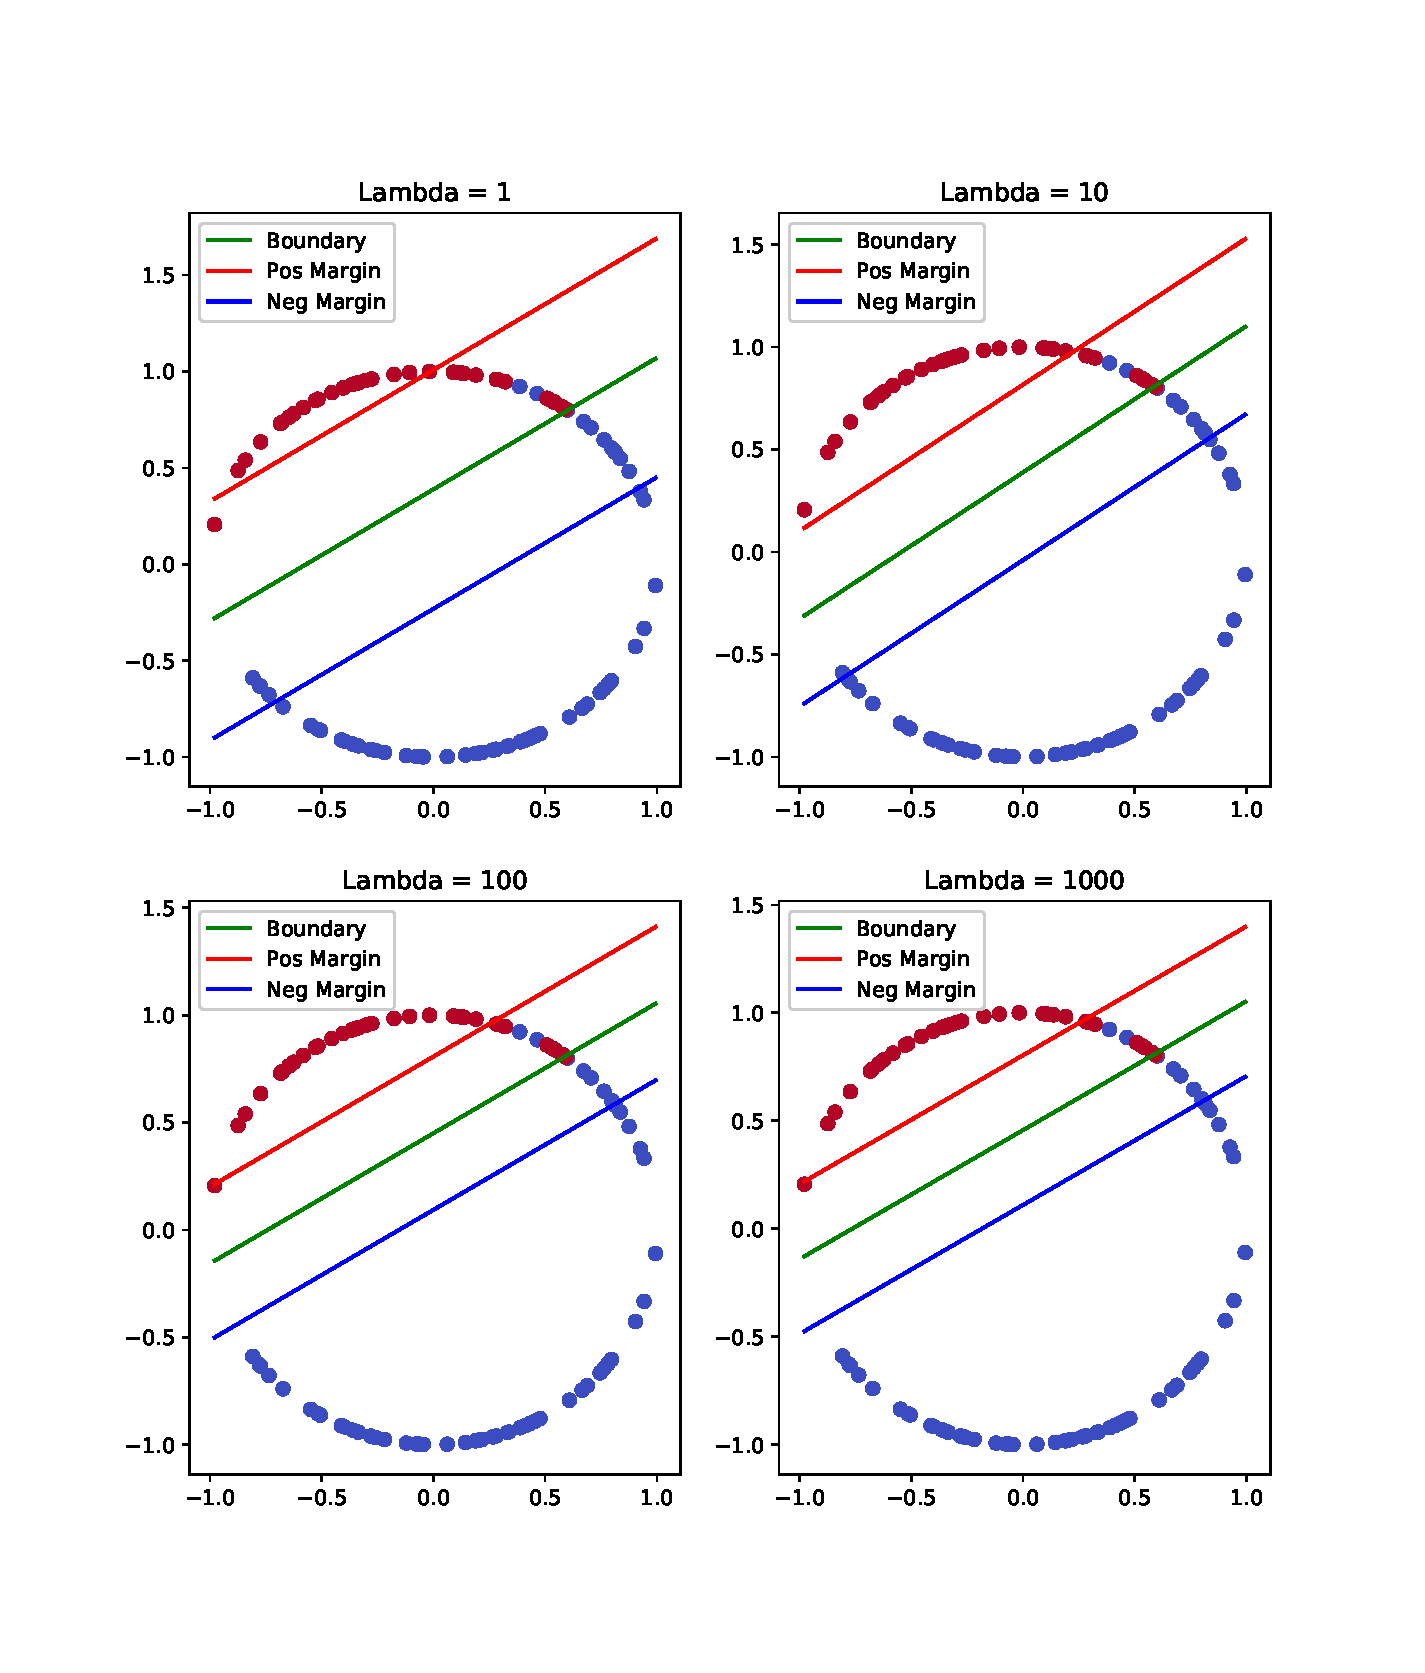
\includegraphics[width=0.8\textwidth]{./img/svm.eps}
	\caption{The Figure of Problem C.b}
	\label{fig:svm}
\end{figure}

(c) \textbf{[4 points]} Report the test error on the test set *test\_data.csv* and *test\_label.csv* for each value of $\lambda$.\\
\textbf{Answer:}\\
\begin{itemize}
	\item $\lambda = 1$: 0.15
	\item $\lambda = 10$: 0.13
	\item $\lambda = 100$: 0.15
	\item $\lambda = 1000$: 0.15
\end{itemize}

(d) \textbf{[4 points]} What is the difference between the result obtained in $\lambda=1$ and $\lambda=10$? Why is that?
\textbf{Answer:}\\
From the figure, we know that the margin area shrinks as the $\lambda$ increases, because higher $\lambda$ will less tolerate the slackness and thus shrink the margin area to remove more points from it. The test error of the SVM with $\lambda=10$ is lower than that with $\lambda=1$; however, this decreasing trend does not hold for the SVMs with $\lambda = 100$ and $\lambda = 1000$.

\newpage

\subsection*{Appendix: Code}


\lstinputlisting[language=Python]{./Python/hw3.py}

\end{document}
